\documentclass{article}
\usepackage{graphicx}
\usepackage{subcaption}

\begin{document}

\begin{figure}[ht]
  \centering
  \begin{subfigure}{0.3\textwidth}
    \centering
    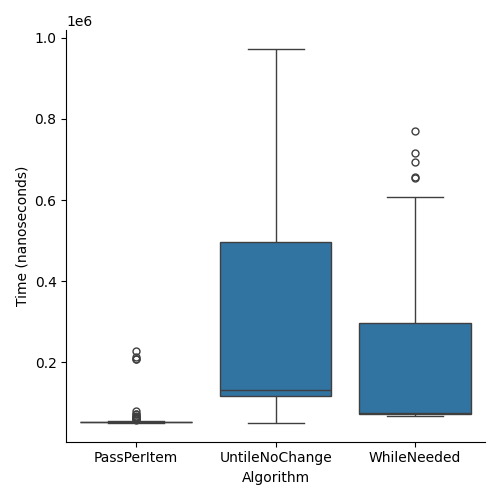
\includegraphics[width=\linewidth]{../figureInt100.png}
    \caption{Size: 100}
    \label{fig:img1}
  \end{subfigure}
  \begin{subfigure}{0.3\textwidth}
    \centering
    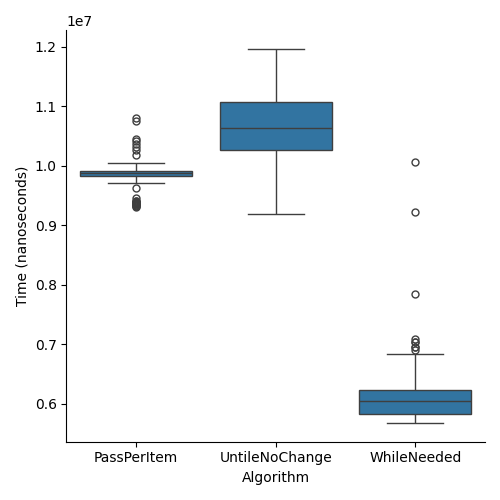
\includegraphics[width=\linewidth]{../figureInt1000.png}
    \caption{Size 1000}
    \label{fig:img2}
  \end{subfigure}
  \begin{subfigure}{0.3\textwidth}
    \centering
    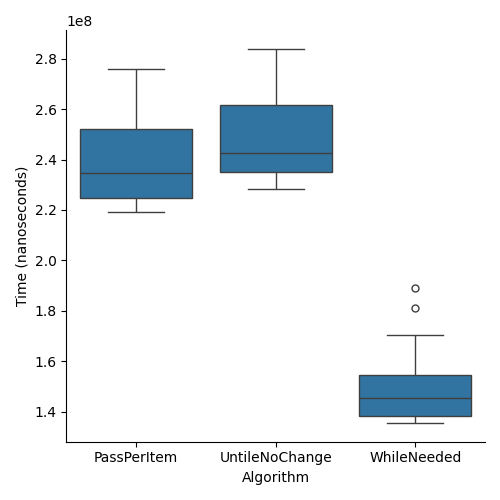
\includegraphics[width=\linewidth]{../figureInt5000.png}
    \caption{Size 5000}
    \label{fig:img3}
  \end{subfigure}
  \caption{Time for sorting array of Integers}
  \label{fig:three_images}
\end{figure}

\begin{figure}[ht]
  \centering
  \begin{subfigure}{0.3\textwidth}
    \centering
    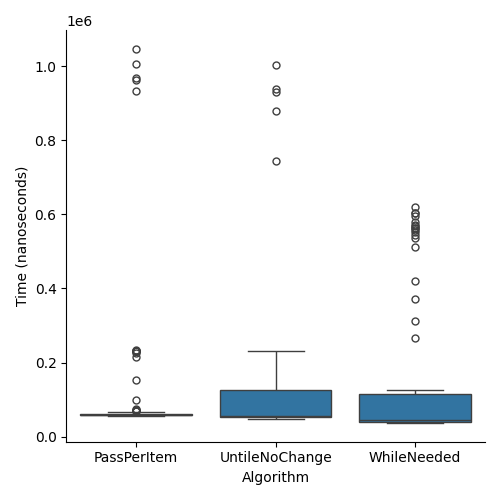
\includegraphics[width=\linewidth]{../figureByte100.png}
    \caption{Size: 100}
    \label{fig:img1}
  \end{subfigure}
  \begin{subfigure}{0.3\textwidth}
    \centering
    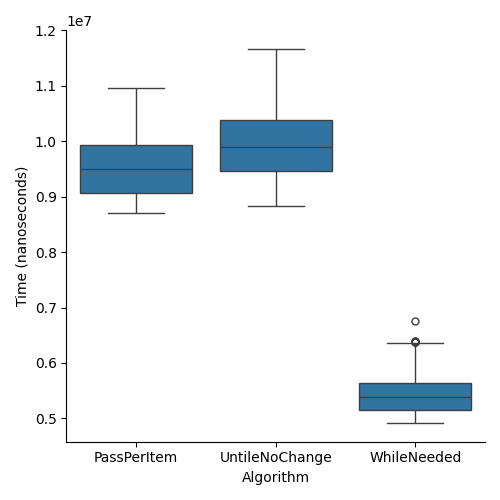
\includegraphics[width=\linewidth]{../figureByte1000.png}
    \caption{Size 1000}
    \label{fig:img2}
  \end{subfigure}
  \begin{subfigure}{0.3\textwidth}
    \centering
    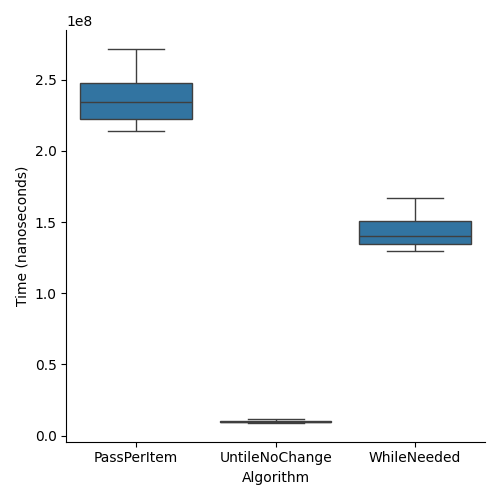
\includegraphics[width=\linewidth]{../figureByte5000.png}
    \caption{Size 5000}
    \label{fig:img3}
  \end{subfigure}
  \caption{Time for sorting array of Bytes}
  \label{fig:three_images}
\end{figure}

\end{document}
